\documentclass[onecolumn, 12pt, a4paper]{article}
\usepackage[margin=1.00in]{geometry}
\usepackage{natbib}
\bibliographystyle{icarus}
\usepackage{amsmath}
\usepackage{amssymb}
\usepackage{subcaption}
\usepackage{graphicx}
\usepackage{caption2}
\usepackage{tabu}
\usepackage{multirow}
\usepackage{siunitx}
\begin{document}



\providecommand{\e}[1]{\ensuremath{\times 10^{#1}}}

\setlength{\parskip}{0em}


\onecolumn{%}
 \centering
 \LARGE Lab 3 Report: Astrometry from CCD Images \\[1.5em]
 %\LARGE Deformation of Mars shorelines explained by Tharsis uplift and limited true polar wander \\[1.5em]
 \large Eden Chen,
        Magdelena Allen, 
        and Joseph Miller

 November 3, 2017
 
 Email: ychen3856@berkeley.edu \linebreak
 Student ID: 3032340806

\vspace{0.25in}

}

\begin{abstract}
In this lab we used the telescope at Leuschner Observatory to track various astronomical objects and their positions in the sky relative to the celestial coordinate system. In this experiment my group and I learned how to use the data collected from the 30-inch telescope to create a digital image of the 25 Phocaea asteroid and find the centroid of its star field. We collected two sets of data from two weeks of observation and we were able to find the asteroid's position by cross matching our image's background stars position with the star field data from the United States Naval Observatory (UNSO) and digital sky survey programs like Aladin. Since the CCD's optical design is limited and only renders a distorted version of the image onto a plane, we will need to calculate the plate constants and the residual amount of distortion. Once we confirmed that our asteroid image matches with the UNSO's data we used linear least squares fit to find the plate constants. We calculated the plate constants between the USNO data and our centroids to be $a_{11} = 1.01263$, $a_{21}$=$-$1.2895$e-2$, $a_{12}$=1.2968$e-2$ and $a_{22}=1.01177$. We also measured our RMS Error to be 0.53 pixel for X and 1.012 pixel for Y. Finally we can use all three epoch observations of the same asteroid to estimate the distance between the asteroid and the Earth or Sun using parallax. We calculated the distance between the Sun and 25 Phocaea to be 1.74 AU on October 11, 2017, 1.87 AU on October 18 and 1.97 AU on October 26, 2017. 25 Phocaea's increase in distance from the Sun suggests that the asteroid is leaving its perihelion.
\end{abstract}

\section{Introduction}  \label{introduction}
Astrometry involves precise measurements of astronomical body and star positions and their motions relative to the celestial coordinate. In this experiment my group and I used a 30-inch telescope located at the Leuschner Observatory in Lafayette, California to obtain three different CCD images of an asteroid. By examining the position of an asteroid with a four-week period we can calculate the asteroid's distance from Earth, its velocity and acceleration. In this experiment my group and I chose to focus on data collected from the asteroid 25 Phocaea. From Lafayette, 25 Phocaea is visible in the evening sky. The asteroid become accessible for observation around 18:00 Pacific Daylight Time (PDT), \ang{55} above the southern horizon. It will continue to be observable until around 22:37, when it sinks to \ang{24} above the western horizon. This asteroid has an semi-major axis of 2.5 Astronomical Unit (AU) with an apparent magnitude of 11.4. We first have to make sure we have located the asteroid by cross matching our CCD image with Aladin and spot the differences. Ideally, our image would contain an extra bright dot near the center compare to the same start field in Aladin, that bright dot would be our asteroid. We will then find the centroids of stars with less than 12.5 apparent magnitude in the CCD image to create a star catalog that we can then used to compare with the USNO catalogs. In order to compare our CCD image we will have to convert the USNO data from Right Ascension and Declination to pixel number. After the comparison we can use the method of linear least squares to determine the plate constants. Finally, we can use the data from the second and third epoch observations to calculate the distance from the Sun to the asteroid and its unit vector by measuring the parallax.

\section{Equipment} \label{Equipment}
In this lab we used a telescope located at the Leuschner Observatory in Lafayette, CA. It is a 30-inch diameter reflecting telescope used for astronomical imaging. The telescope uses a SBIG ST-L-11K camera which contains a Kodak KAI-11000M $4008 \times 2762$ pixel CCD array. The output field of view is approximately 12 arc minutes $\times$ 15 arc minutes. The complete specifications of the telescope are listed in the table below:  \newline

\centerline{
\begin{tabu} to 1\textwidth { | X[l] | X[r] | }
 \hline
 Site & Russell Reservation Lafayette, CA \\
 \hline
 Geographic location  & \ang{37}55' 06''N \ang{121}09'24''W \\
\hline
 Primary mirror & Nominal 30-inch in diameter F/2.5\\
 \hline
 Optical recipe  & $R_1 = 150.0$ inch $R_2 = -65.278$ inch, $d_{12} = 52.560$ inch \\
\hline
 Magnification & m = s'/s = 3.2\\
 \hline
 System F/ratio-focal length  & F/8 - 6096 mm (33.84 arc sec/mm) \\
 \hline
 Camera & SBIG ST-L-$11K^3$ \\
 \hline
 Detector  & KAI-11000M, TE cooled CCD \\
 \hline
 CCD format & $4008 \times 2672$, \SI{9}{\micro\metre} pixels \\
 \hline
 Nominal pixel scale  & 0.30 arc seconds/pixel (unbinned) \\
 \hline
 Field-of-view & $12 \times 15$ arc minutes \\
 \hline
 Optical Filters  & BVRI \\
\hline
 Limiting Magnitude & R = 16/17 mag. (1/6 seconds) \\
\hline
\end{tabu}}
\leavevmode
\newline
\newline
\centerline{
Table 1: The specifications of the telescope used for this lab experiment.
}
\newline

\section{Acquiring Data} \label{AD}
In this lab we will need three epoch observations with a week in between each collection in order to construct a model for velocity and acceleration measurement. On October 18, 2017, under the guidance of graduate student instructor Jordan Sligh, Elena, Joe and I collected our first set of CCD images of 25 Phocaea. We collected eight sets of 25 Phocaea and dark current images with the exposure time of 32 seconds and we will choose one set to be our second epoch observation. For the first and third epoch observation we will have to use the data collected by other lab groups. We decided to use one set of data collected by the group Starbursts on October 11, 2017 with eight seconds exposure time to be our first epoch observation. For the third epoch observation we chose one set of 25 Phocaea and dark current data collected on October 26, 2017 with eight seconds exposure time. \newline


\hspace*{-.8cm}\begin{tabular}{ |p{2cm}|p{2.5cm}|p{2cm}|p{2.3cm}|p{2.3cm}|p{2.5cm}|p{1.3cm}| }

 \hline
 Local Date & Target Name & Exposure Time (s)& RA(2000) HH:MM:SS & DEC(2000) $\pm$DD:MM:SS & Focus (\SI{}{\micro\metre})\\
 \hline
 10-11-2017 & 25 Phocaea & 8& 20:50:23 & +09:00:12 & 25814.1\\
 \hline
 10-18-2017 & 25 Phocaea & 32& 21:00:25 & +07:19:35 & 25811.3\\
 \hline
 10-26-2017 & 25 Phocaea & 8& 21:11:56 & +05:35:14 & 25806.8\\
 \hline
\end{tabular}

\leavevmode
\newline

\centerline{Table 2: Three chosen sets of data taken on a weekly basis.}
\section{Data Processing}
For data processing I will focus on the 25 Phocaea data collected on October 18, 2017 with 32 seconds exposure time. The KAI-11000M CCD generate images with 4008 $\times$ 2672 pixels. The resultant FITS files would be too large to be practically worked on so we reduced the size of the image by binning two pixels into one. The binning mode in the CCD halved the size of the image from 4008 $\times$ 2672 to 2004 $\times$ 1336 pixels. The reason CCD images with high exposure time are great to work with is because we can see more dimmer stars that can help us recognize patterns in the star field easier. Here is the raw CCD image rotated \ang{90} counterclockwise:

\begin{subfigure}{\linewidth}\hspace*{-1.cm}
  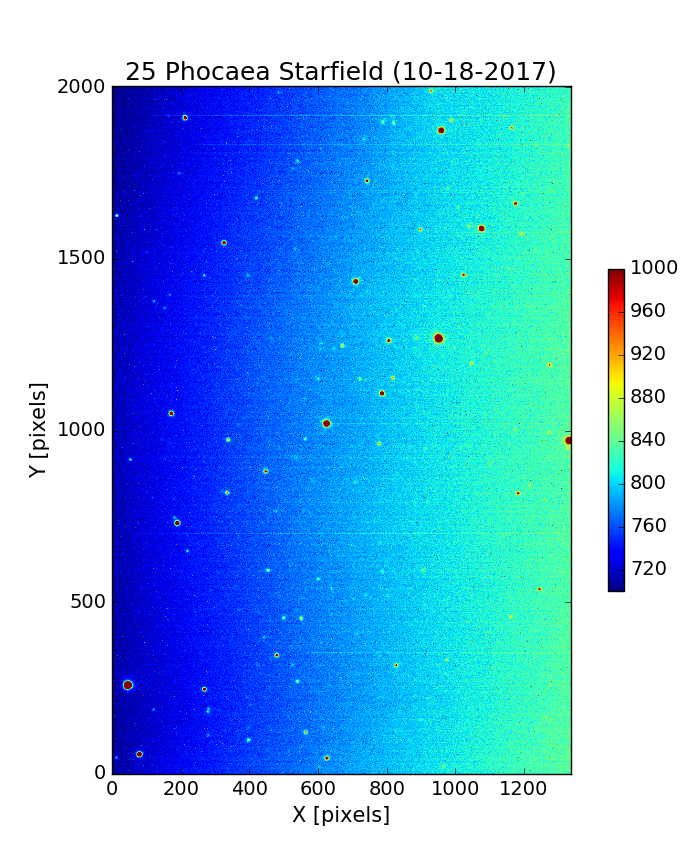
\includegraphics[width=.5\linewidth]{figure_1.png}
  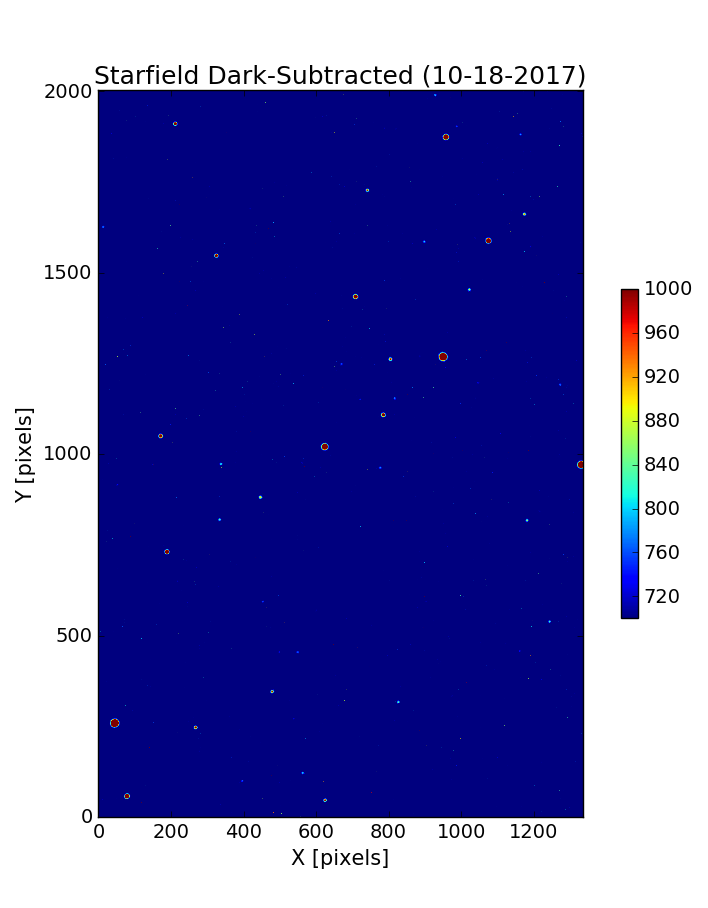
\includegraphics[width=.485\linewidth]{figure_1-1.png}
  \end{subfigure}\par\medskip


\newline
Figure 1: Left: The raw image of the field centered at RA = 21:00:25 DEC = +07:19:35. This image is generated by the CCD in the telescope with 32 seconds exposure time. Notice there is a strong bias gradient from left to right that will need to be eliminated by subtracting out the dark current. Right: Same image as the left but with the bias and dark current subtracted out.

\centerline{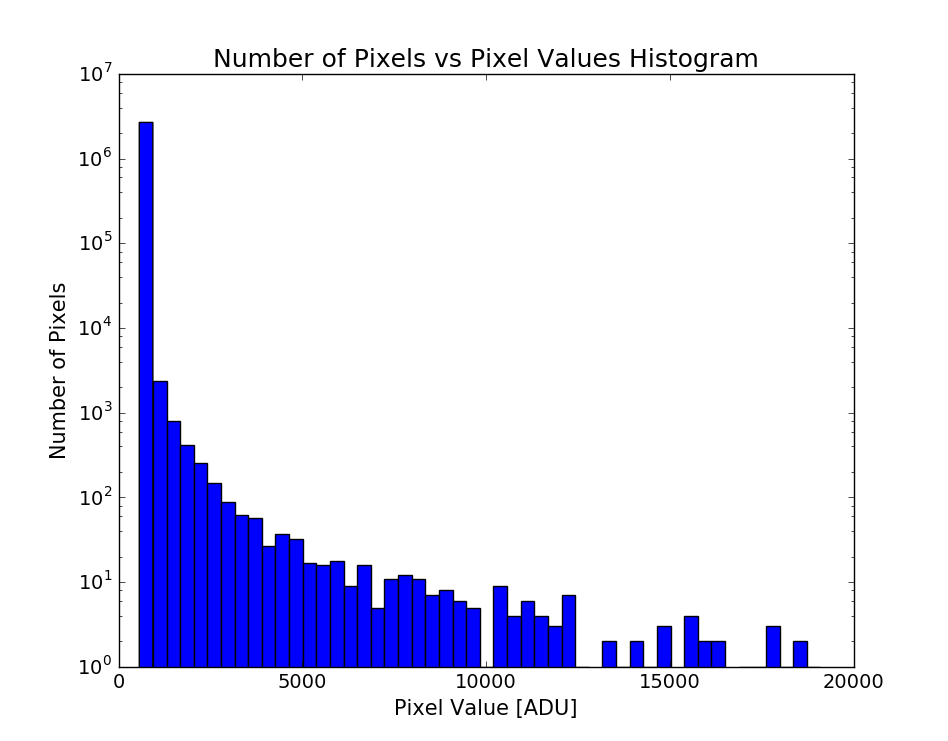
\includegraphics[scale=.37]{figure_1-2.png}}
\newline
Figure 2: We can also create a histogram to see the grouping of pixels with their respective pixel values. We can see that most pixels have the pixel value of less than 1000 counts. 
\newline
\newline
The histogram helped us better visualize the average pixel value of a specific image. We can now modify Figure 1 by limiting the image to scale on a range of pixel value between 700 to 1000 counts:

\centerline{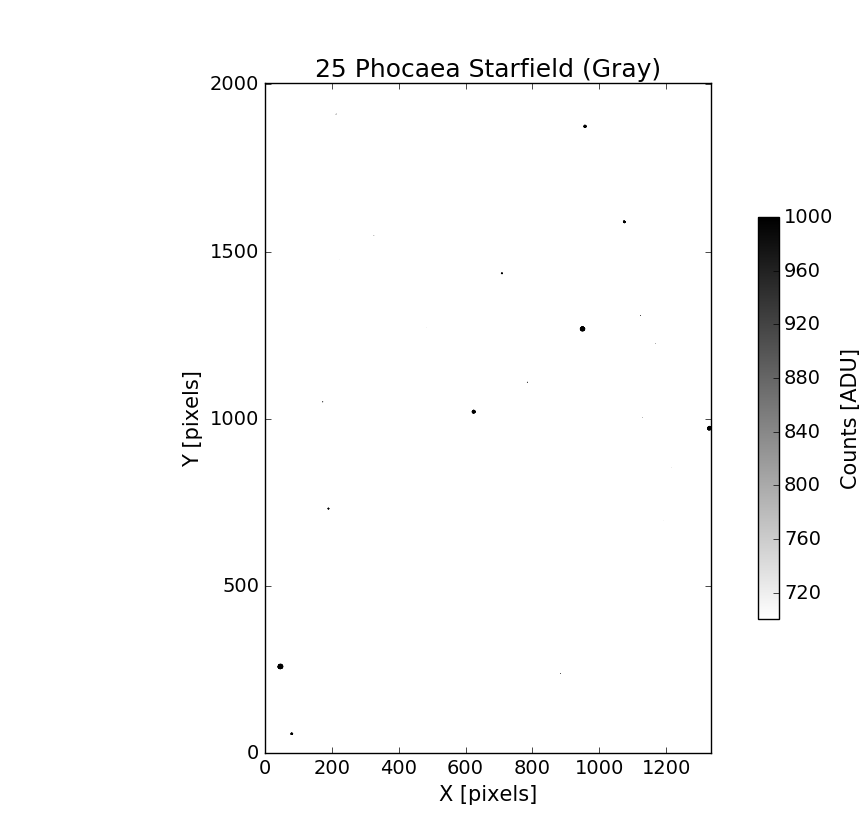
\includegraphics[scale=.5]{figure_1-3.png}\hspace*{1.6cm}}
\newline

Figure 3: Same image as Figure 1 in inverse color. This image is also better at displaying dimmer stars because we lowered the pixel value range. The color bar on the right shows the range of pixel values mapped to grey levels.
\newline

\section{Star Positions and Catalogs}
After we clear up the image and confirm that the telescope was pointed at the correct position we can locate the star positions by measuring their x- and y-positions. The location of stars are best measured using their centroids. Centroids of the stars can be measured by using \newline
\begin{equation}\label{eq:1}
<x> = \sum_{i=j}{X_i I_i }/ \sum_{i=j}{I_i}
\end{equation}
\leavevmode
\newline
where the summation i only runs over a region in the vicinity of the star. $\sum_{}{I_i}$ is a singular measurement of the brightness of the star. We first locate the pixel positions of 16 brightest objects and circles them. Then, we can calculate the centroid locations:

\begin{subfigure}{\linewidth}\hspace*{-2.5cm}
  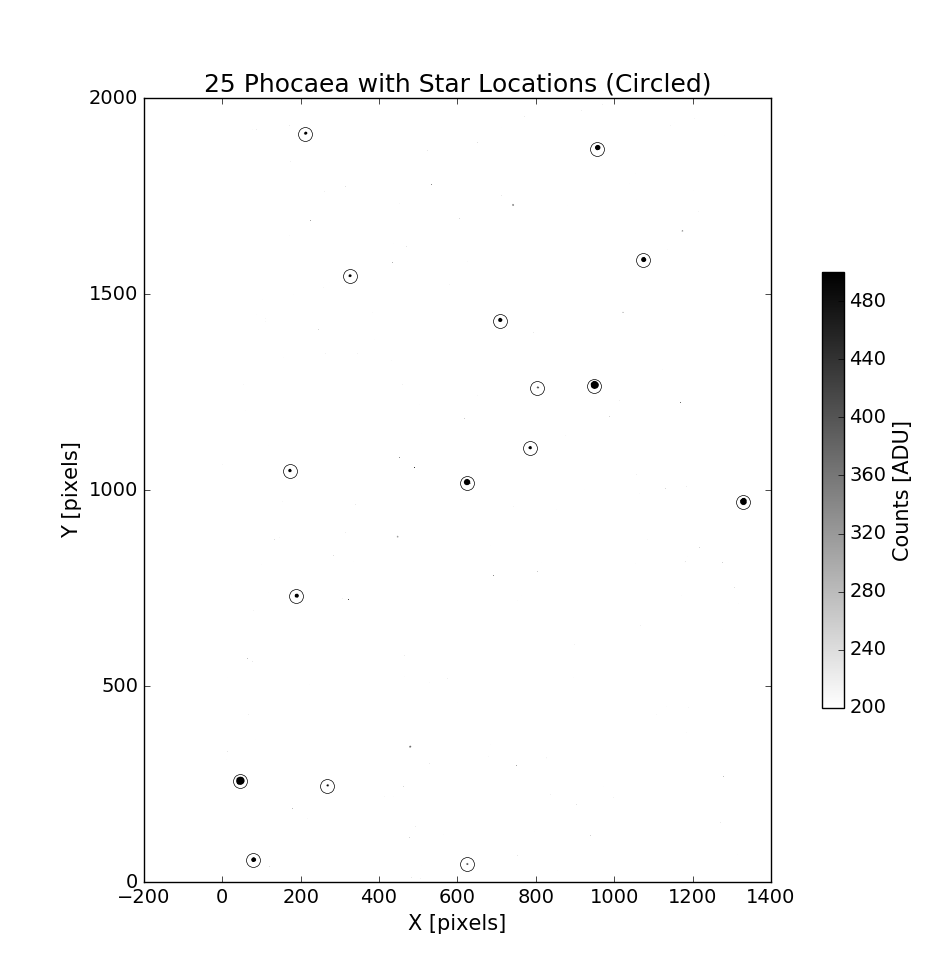
\includegraphics[width=.56\linewidth]{figure_2.png}
  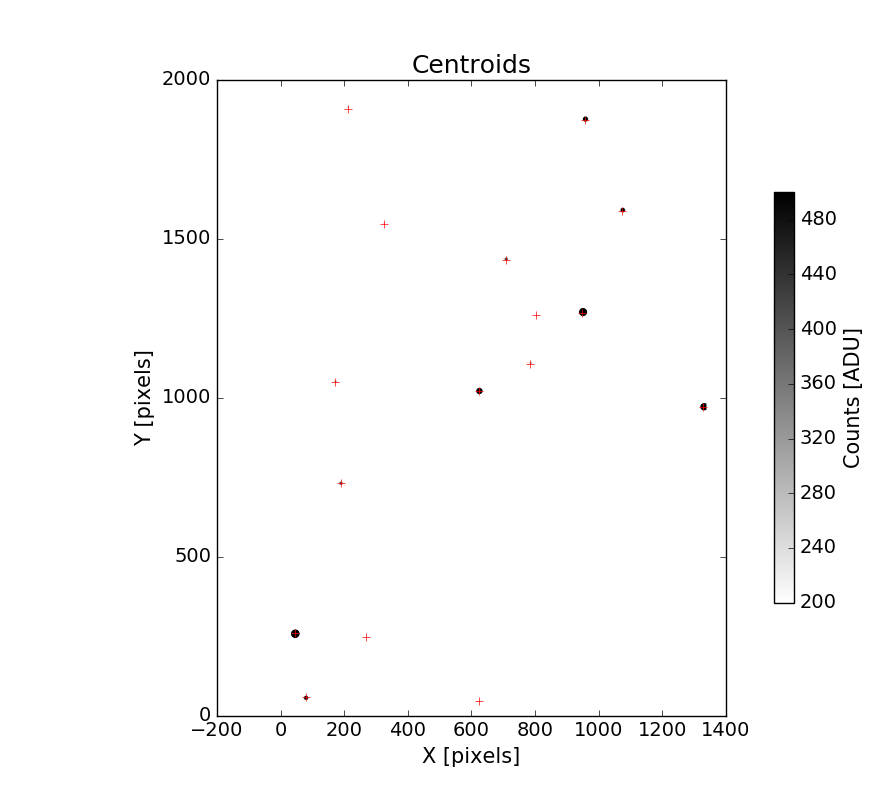
\includegraphics[width=.64\linewidth]{figure_1-4.png}
  \end{subfigure}\par\medskip

\newline

Figure 4: Left: The R-band image of 25 Phocaea from Figure 3. The circles show the position of the 16 brightest objects, it is found by computing the brightest pixel and calculate the center of light and repeat to find the next one. Notice that there are one extra circle at the center of the image, that is our asteroid. Right: The same figure but with centroids displayed as red crosses.
\newline
 
After we have the centroid plot we want to fetch the data from USNO at RA 21:00:25 and DEC +07:19:35 and compare the two. We can get the data by using the web-based Vizier astronomical catalog system. The data we get from USNO will be in units of degrees and we need to convert them to pixel positions. For an ideal camera, the conversion can be done with the following equations:\newline

\begin{equation}\label{eq:2}
x = f(X/p)+x_0 
\end{equation}
\begin{equation}
y = f(Y/p)+y_0
\end{equation}
where 
\begin{equation}\label{eq:4}
X = - \dfrac{cos\delta sin(\alpha - \alpha_0)}{cos\delta_0 cos\delta cos(\alpha - \alpha_0) + sin\delta sin\delta_0}
\end{equation}
\begin{equation}\label{eq:4}
Y = - \dfrac{cos\delta_0 cos\delta cos(\alpha - \alpha_0)-cos\delta_0 sin\delta}{cos\delta_0 cos\delta cos(\alpha - \alpha_0) + sin\delta sin\delta_0}
\end{equation}\label{eq:5}
\newline

X and Y makes up the projected coordinates (X, Y) of a position on the celestial sphere ($\alpha$, $\delta$) in the vicinity of a field centered at ($\alpha_0$, $\delta_0$). The $f$ is the focal length of the camera (6300mm) and p is the pixel size (0.018mm). $x_0$ and $y_0$ are the offset pixel numbers.
\newline

\begin{subfigure}{\linewidth}\hspace*{-1.5cm}
  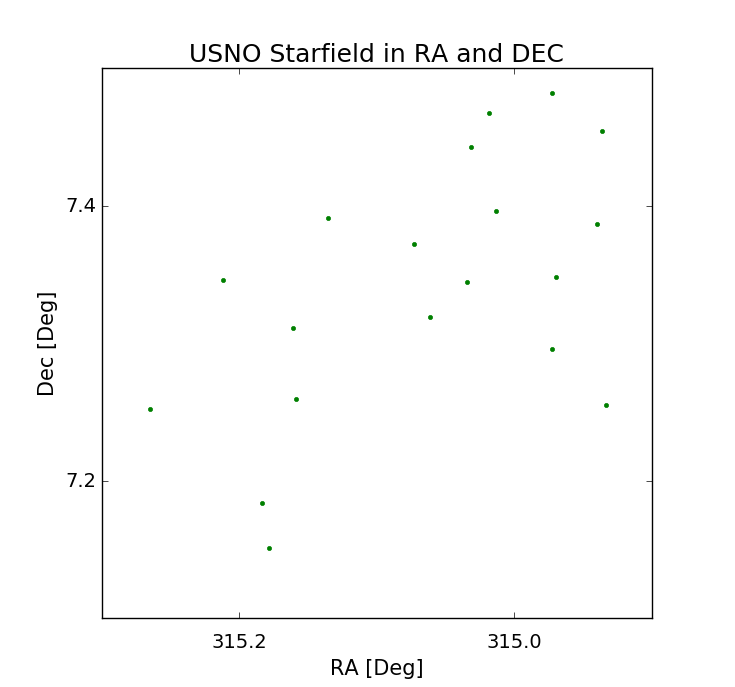
\includegraphics[width=.55\linewidth]{figure_1-5.png}
  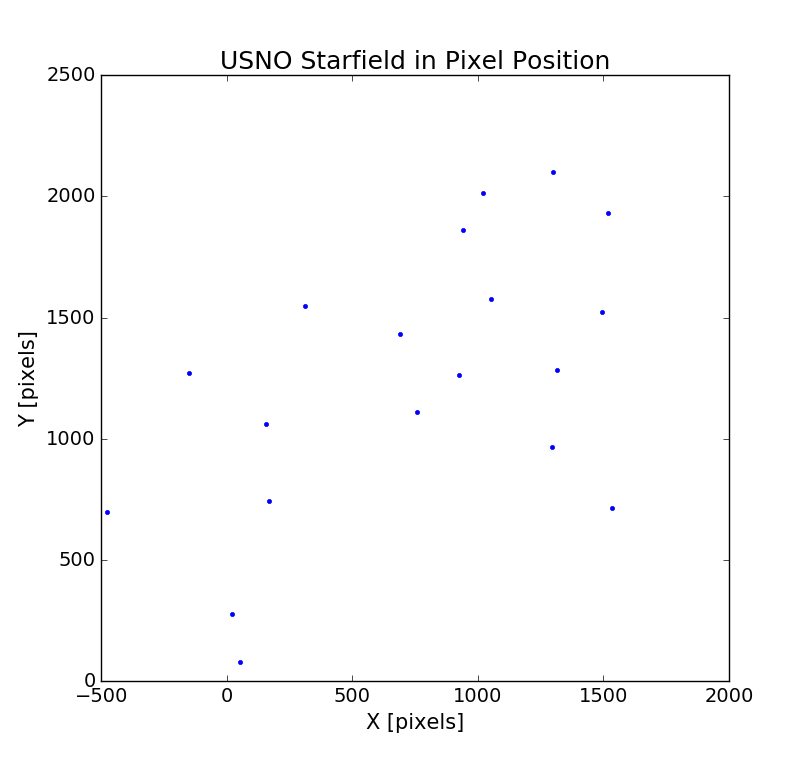
\includegraphics[width=.55\linewidth]{figure_1-6.png}
  \end{subfigure}\par\medskip

\newline
Figure 5: Left: The USNO starfield with RA 21:00:25 and DEC +07:19:35 in degrees. Right: USNO starfield data converted to pixel positions. \newline

Once we have the USNO data in pixel positions, we can compare our centroid plot with it:

\centerline{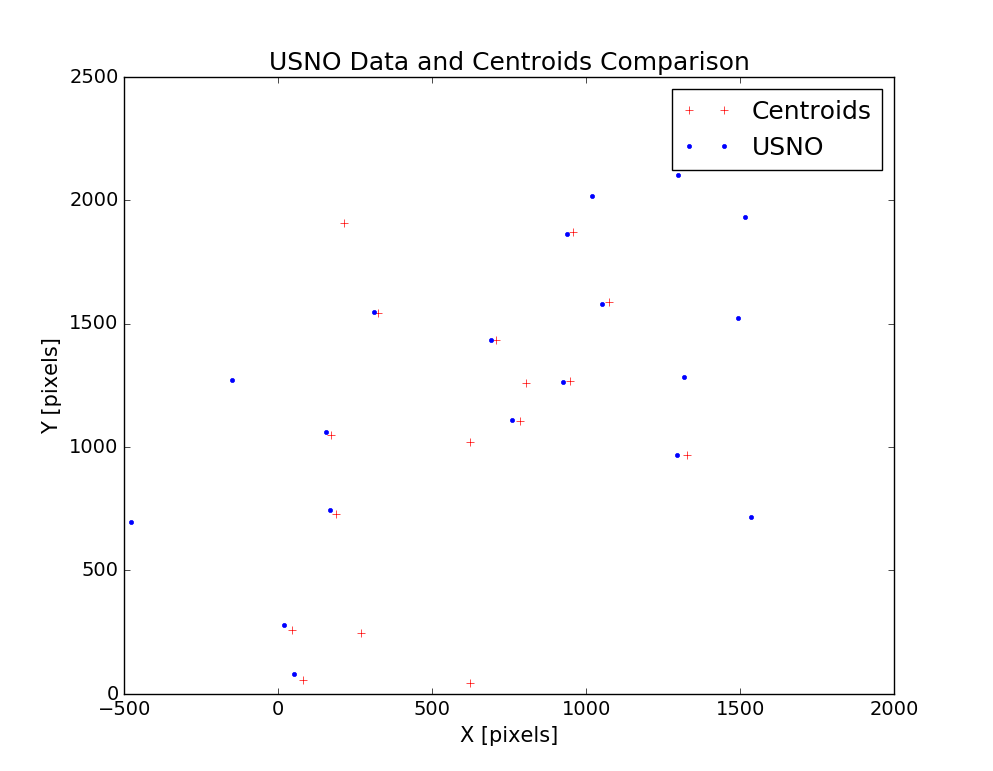
\includegraphics[scale=.4]{figure_1-7.png}}

Figure 6: The USNO data in comparison with our centroid plot. We can see that there are up to 11 centroid positions matches up with the USNO data and confirm that we are looking at the right direction. \newline

\section{Plate Constants and RMS Error}
Once we located a number of centroids matches the USNO catalog we can use linear least squares to find the plate constants and calculate the Root Mean Square (RMS) error. RMS error is the standard deviation of the residual (prediction errors) caused by variable magnification and distortion from the CCD's optical system. We can get the plate constants by using linear transformation. This transformation can be done by doing matrix multiplication with homogeneous coordinates: \textbf{x = TX} where \textbf{X} = (X, Y, 1), \textbf{x} =(x, y, 1) and

\begin{equation}\label{eq:1}
\textbf{T} = 
\left(\begin{array}{ccc} (f/p)a_{11} & (f/p)a_{12} & x_{0}\\ (f/p)a_{21} & (f/p)a_{22}\\ 0&0&1 \end{array}\right)
\end{equation}

\leavevmode
\newline
The plate constants can then be found by using the condition describing the relation between the independent variables and the number of position measurements of the dependent variable from the CCD image. This can be written in a compact form of \textbf{a} = \textbf{Bc} where \newline

\hspace*{4cm}{
\begin{equation}\label{eq:2}
\textbf{a} =
\left(\begin{array}{ccc} x_1 \\ x_2 \\ ... \\ x_N \end{array}\right)
, \textbf{B} = 
\left(\begin{array}{ccc} (f/p)X_1 & (f/p)Y_1 & 1 \\ (f/p)X_2 & (f/p)Y_2 & 1 \\ ... & ...& ... \\ (f/p)X_N & (f/p)Y_N & 1 \end{array}\right)
, \textbf{c} =
\left(\begin{array}{ccc} a_{11} & a_{12} & x_0 \end{array}\right)
\end{equation}}

\leavevmode
\newline
\newline
\textbf{a} is an array of x-axis pixel positions of USNO stars that are in pair with our centroid positions. By using the relation between Eq.(6), Eq.(7) and 

\begin{equation}
\textbf{c} = (\textbf{B}^{T}\textbf{B})^{-1}\textbf{B}^{T}\textbf{a}
\end{equation}

\leavevmode
\newline
we found the plate constants listed in Table 3:
\newline

\hspace*{2cm}{
\begin{tabu} to .7\textwidth { | p{2cm} | p{3.5cm}| p{3.5cm}| }
 \hline
 &X & Y \\
 \hline
 &$a_{11}$=1.01263 & $a_{21}$=$-$1.2895$e-2$ \\
 \hline
 &$a_{12}$=1.2968$e-2$ & $a_{22}$=1.01177\\
\hline
 RMS Error &0.53 pix & 0.49 pix \\
 \hline
 $\sqrt{det(T)}$ & 1.012 & 1.012\\
 \hline
\end{tabu}
}
\leavevmode
\newline
\newline
\newline
Table 3: The least squares coefficients assuming $f$=6300mm and $p$=0.018mm. The RMS Error for X is 0.53 pixel and 0.49 pixel for Y. $\sqrt{det(T)}$ is the effective telescope scale f/p in pixels per radians.\newline

Once we have the RMS error we can use eight best matching pair of stars between the USNO data and our centroids for the linear least-squares fit. We can plot the result and see the pixel separation between each matching pair.


\centerline{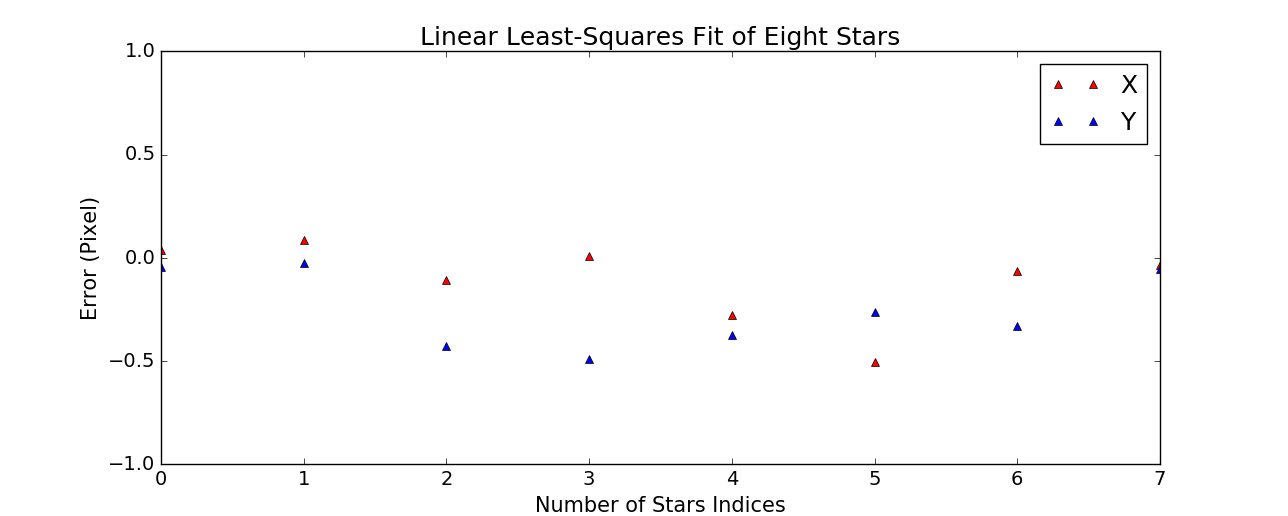
\includegraphics[scale=.5]{figure_1-8.png}}
\leavevmode
\newline
Figure 7: Eight best matching stars extracted from Figure 6 and have been used in a linear least-squares fit. This figure consntructed by the plate constants we calculated and the RMS error of x is 0.53 pixels and RMS error of y is 0.49 pixels. 

\section{Measuring Parallax}
After we compare our centroids and the USNO starfield, we pick out the centroids without matching stars and convert the rest of the pairs in pixel coordinate to projected coordinates and then to RA and DEC. By examining Figure 3 and compare it with Aladin digital sky survey at the same RA and DEC we can spot the difference in number of bright objects and identify our asteroid. For the second epoch we calculated the true RA and DEC of 25 Phocaea to be 21:08:17 and +07:27:49. We can do the same for the first and third epoch observation and construct a new table: \newline

\hspace*{-.5cm}\begin{tabular}{ |p{2cm}|p{2.5cm}|p{2cm}|p{2.3cm}|p{2.3cm}|p{2.5cm}|p{1.3cm}| }

 \hline
 Local Date & Target Name & Exposure Time (s)& RA(2000) HH:MM:SS & DEC(2000) $\pm$DD:MM:SS & Focus (\SI{}{\micro\metre})\\
 \hline
 10-11-2017 & 25 Phocaea & 8 & 20:58:48 & +09:12:05 & 25814.1\\
 \hline
 10-18-2017 & 25 Phocaea & 32 & 21:08:17 & +07:27:49 & 25811.3\\
 \hline
 10-26-2017 & 25 Phocaea & 8 & 21:20:16 & +05:45:56 & 25806.8\\
 \hline
\end{tabular}
\leavevmode
\newline

Table 4: A more precise version of Table 2 with more accurate sets of 25 Phocaea location in RA and DEC.

\leavevmode
\newline
We first want to find the unit vectors from the Earth to the asteroid in terms of \textbf{s}, then we can use 

\begin{equation}\label{}
\rho s =
\left(\begin{array}{ccc} x_{eq} - X_{eq} \\ y_{eq} - Y_{eq} \\ z_{eq} - Z_{eq} \end{array}\right)
= \rho
\left(\begin{array}{ccc} cos\alpha cos\delta \\ sin\alpha cos\delta \\ sin\delta \end{array}\right)
\end{equation}
\newline

where $\alpha$ is the asteroid's RA in radiant and $\delta$ is DEC in radiant and \textbf{s} is the unit vector from Earth to the Asteroid. Three epoch observations will produce three sets of \textbf{s}: \newline

\hspace*{-.5cm}\begin{tabular}{ |p{1cm}|p{2.5cm}|p{2.5cm}|p{2.3cm}|p{2.3cm}|p{2.5cm}|}

 \hline
  & $\textbf{s}_x$ & $\textbf{s}_y$ & $\textbf{s}_z$ & HH:MM:SS & DEC(2000) $\pm$DD:MM:SS\\
 \hline
 $\textbf{s}_1$ & 0.69434367 & $-0.70165316$ & 0.15990531 & 20:58:48 & +09:12:05\\
 \hline
 $\textbf{s}_2$ & 0.72599242 & $-0.6753236$ &  0.1298963 & 21:08:17 & +07:27:49 \\
 \hline
 $\textbf{s}_3$ & 0.76291317 & $-0.63864818$ & 0.10045896 & 21:20:16 & +05:45:56 \\
 \hline
\end{tabular}
\newline
\newline

Table 5: Unit vectors of the distance between Earth and the asteroid from three epoch observations and their vector components  $\textbf{s}_x$,  $\textbf{s}_y$ and  $\textbf{s}_z$. \newline

We can now calculate the scalar distance $\rho$ in AU between the Earth and the asteroid of each epoch observations using \newline

\begin{equation}\label{}
\rho = k^2(\dfrac{1}{R^3} - \dfrac{1}{r^3}) \dfrac{\dot{s}\cdot(\textbf{R}\times\textbf{s})}{\dot{s}\cdot(\ddot{s}\times\textbf{s})}
\end{equation}
\newline

and 
\begin{equation}\label{}
r^2 = \rho^2 + R^2 + 2\rho\textbf{R}\cdot\textbf{s}
\end{equation}
\newline
Where \textbf{R} is the unit vector from the Sun to the Earth and there will be three $\rho$s representing the Sun-Earth coordinate at three different times and R is their scalar distance, which is roughly one AU. $\dot{s}$ is the velocity vector and $\ddot{s}$ is the acceleration vector of the asteroid. \newline

\hspace*{-1.2cm}\begin{tabular}{ |p{2.5cm}|p{2.5cm}|p{2.5cm}|p{2.5cm}|p{2.3cm}|p{2.5cm}|}

 \hline
  $\textbf{R}$ and Date (PDT)& $\textbf{R}_x$(Pixel) & $\textbf{R}_y$(Pixel) & $\textbf{R}_z$(Pixel) & HH:MM:SS & DEC(2000) $\pm$DD:MM:SS\\
 \hline
 $\textbf{R}_1$(10-11-2017) & 9.4218496$e-1$ & 3.1244318$e-1$ & 1.3529976$e-1$ & 20:58:48 & +09:12:05\\
 \hline
 $\textbf{R}_2$(10-18-2017)& 8.9303099$e-1$ &  4.1370035$e-1$  & 1.7919212$e-1$ & 21:08:17 & +07:27:49 \\
 \hline
 $\textbf{R}_3$(10-26-2017)& 8.2084150$e-1$ & 5.2196548$e-1$ & 2.2612882$e-1$ & 21:20:16 & +05:45:56 \\
 \hline
\end{tabular}
\leavevmode
\newline
\newline

Table 6: The Sun-Earth unit vectors and their respective date and RA and DEC in pixel positions. (Source: https://ssd.jpl.nasa.gov/horizons.cgi)
\newline

To find a precise distance between the Sun and the asteroid we will need to have an initial guess of r and start plugging into Eq.(10) and then plug the resultant $\rho$ into Eq.(11) and repeat. Eventually $\rho$ and r will converge to a number in AU. We calculated our $\rho$ and r in Table 7:\newline

\hspace*{.5cm}\begin{tabular}{ |p{2.5cm}|p{2.5cm}|p{2.5cm}|p{2.3cm}|p{2.3cm}|}

 \hline
  Date(MM-DD-YYYY)& r (AU) & $\rho$ (AU) & HH:MM:SS & DEC(2000) $\pm$DD:MM:SS\\
 \hline
 10-11-2017 & 1.7457869 & 1.0454778 & 20:58:48 & +09:12:05\\
 \hline
 10-18-2017 & 1.8722276 & 1.2384398 & 21:08:17 & +07:27:49 \\
 \hline
 10-26-2017 & 1.9685838 & 1.4092013 & 21:20:16 & +05:45:56 \\
 \hline
\end{tabular}
\newline
\newline

Table 7: The calculated distances between the Sun and the asteroid r (AU) and distances between the Earth and the asteroid $\rho$ (AU) with their respective RA and DEC for all three epochs. \newline

Finally we want to calculate the respective unit vector for r by using 
\newline
\begin{equation}
    \textbf{r} = \textbf{R} + \rho\textbf{s}
\end{equation}
where the \textbf{r} is the unit vector from the Sun to the asteroid, \textbf{R} is the Sun-Earth unit vectors from Table 6. \newline

\hspace*{-1.2cm}\begin{tabular}{ |p{2.5cm}|p{2.5cm}|p{2.5cm}|p{2.5cm}|p{2.3cm}|p{2.5cm}|}

 \hline
  $\textbf{r}$ and Date (PDT)& $\textbf{r}_x$(Pixel) & $\textbf{r}_y$(Pixel) & $\textbf{r}_z$(Pixel) & HH:MM:SS & DEC(2000) $\pm$DD:MM:SS\\
 \hline
 $\textbf{r}_1$(10-11-2017) & 1.6681058 & $-0.4211196$ & 0.3024772 & 20:58:48 & +09:12:05\\
 \hline
 $\textbf{r}_2$(10-18-2017)& 1.7921288 & $-0.4226473$  & 0.3400608 & 21:08:17 & +07:27:49 \\
 \hline
 $\textbf{r}_3$(10-26-2017)& 1.8959397 & $-0.3780184$ & 0.3676957 & 21:20:16 & +05:45:56 \\
 \hline
\end{tabular}
\leavevmode
\newline

Table 8: The unit vector of the distance between the Sun and the asteroid in pixel positions calculated from Eq.(12) and their respective dates and RA and DEC.
\newline
\section{Conclusion and Discussion}
In this lab we used the 30-inch telescope located at Leuschner Observatory in Lafayette, CA to take three separate images of the asteroid 25 Phocaea at three different times with each data taken at a week apart. We locate the asteroid by computing the plate constants and the RMS error in order to compare our centroids with the USNO star field. The resultant RMS errors in x and y pixel positions can be used to adjust our initial RA and DEC to the true position of the asteroid. We can then convert the true RA and DEC to unit vectors $\textbf{s}$ of the distance between the Earth and the asteroid using Eq.(9). By consulting the Sun-Earth unit vector data from Table 6 we calculated the scalar distance $\rho$ from the Earth to the asteroid using Eq.(10). The scalar distance $\textbf{r}$ can be precisely measured by repeat calculation between Eq.(9) and Eq.(10). Table 7 showed the calculated r (AU) and $\rho$ (AU). We then calculated the unit vector $\textbf{r}$ by using Eq.(12) and the results are shown in Table 8. There is a trend in Table 7 showing that the asteroid is moving farther away from the sun each week. This data suggests that the asteroid is moving away from its perihelion around the Sun and possibly decelerating. 
\end{document}